\documentclass[12pt, spanish]{article}
\usepackage[spanish]{babel}
\selectlanguage{spanish}

% estilo personalizado
\usepackage{src/estilo}


\begin{document}

% Página de titulo

%%%%%%%%%%%%%%%%%%%%%%%%%%%%%%%%%%%%%%%%%%%%%%%%%%%%%%%%%%%%%%%%%%%%%%%%%%%%%%%%%%%%%%%%%

\begin{titlepage}
    \centering
    \vspace*{-2cm}
    
\includegraphics[scale = 0.50]{ugr.png}\\[0.3 cm]
    %\textsc{\LARGE Universidad de Granada}\\[2.0 cm]
    \textsc{\large Introducción a la Programación para Ciencia de Datos}\\[0.5 cm]
    \textsc{\large Master en Ciencia de Datos e Ingeniería de Computadores}\\[0 cm]
    \rule{\linewidth}{0.2 mm} \\[0.4cm]
    { \Large \bfseries \thetitle}\\
    \rule{\linewidth}{0.2 mm} \\[1 cm]

     {\large
      \emph{Autor: } \theauthor\\
	   \emph{DNI:   }  77021623-M \\
      \emph{Correo:} advy99@correo.ugr.es}

	 
\includegraphics[scale = 0.20]{logo_etsiit.png}\\[0.3 cm]
    {\large \thedate}\\[0.75cm]
	 \url{https://github.com/advy99/IPCD/}\\[0.75cm]
    \doclicenseThis
\end{titlepage}



\pagestyle{fancy}


%%%%%%%%%%%%%%%%%%%%%%%%%%%%%%%%%%%%%%%%%%%%%%%%%%%%%%%%%%%%%%%%%%%%%%%%%%%%%%%%%%%%%%%%%

% indice

\tableofcontents
\pagebreak

%%%%%%%%%%%%%%%%%%%%%%%%%%%%%%%%%%%%%%%%%%%%%%%%%%%%%%%%%%%%%%%%%%%%%%%%%%%%%%%%%%%%%%%%%

% secciones

\section{Introducción}

En este trabajo resolveremos un problema de clasificación utilizando el lenguaje de programación Python. En concreto utilizaremos las distintas técnicas de preprocesamiento, selección de hiperparámetros y aprendizaje automático disponibles en el paquete scikit-learn, así como otras bibliotecas para diversas tareas entre las que se encuentran visualizar gráficamente el conjunto de datos, guardar los modelos obtenidos en disco, entre otras tareas.

En concreto, los módulos utilizados son:

\begin{itemize}
	\item \texttt{os}: Realizar tareas del sistema operativo, como crear carpetas.
	\item \texttt{sys}: Gestionar parámetros específicos del sistema.
	\item \texttt{pandas}: Leer ficheros de disco en forma de DataFrames.
	\item \texttt{seaborn}: Herramienta para realizar gráficas.
	\item \texttt{matplotlib}: Herramienta para realizar gráficas.
	\item \texttt{numpy}: Herramientas de computación numérica.
	\item \texttt{pickle}: Almacenar variables de Python en disco.
	\item \texttt{sklearn}: Herramientas de aprendizaje automático.
\end{itemize}

\newpage


\section{Problema a resolver}

En este trabajo se intentará resolver el problema de clasificación del conjunto de datos South German Credit. Este conjunto de datos cuenta con 21 variables, siendo la última de estas la variable a predecir. La variable a predecir se trata de una variable lógica, sobre si se ha cumplido o no los pagos del crédito concedido.

Este conjunto de datos cuenta con información sobre la persona que solicita el crédito, por ejemplo el estado de la cuenta bancaria, si ha cumplido o no con los pagos de otros créditos con anterioridad, el trabajo, la edad, entre otras variables, y debido a la gran cantidad de estas, se aplicará un análisis de componentes principales (PCA) de cara a reducir la dimensionalidad del problema.

Para entender de una mejor forma el conjunto de datos, se han realizado distintas gráficas para mostrar el comportamiento de cada predictor.

Lo primero que tenemos que tener en cuenta para un problema de clasificación es si el problema está balanceado, es decir, contamos con un número similar de observaciones de cada clase:

\begin{figure}[H]
	\centering
	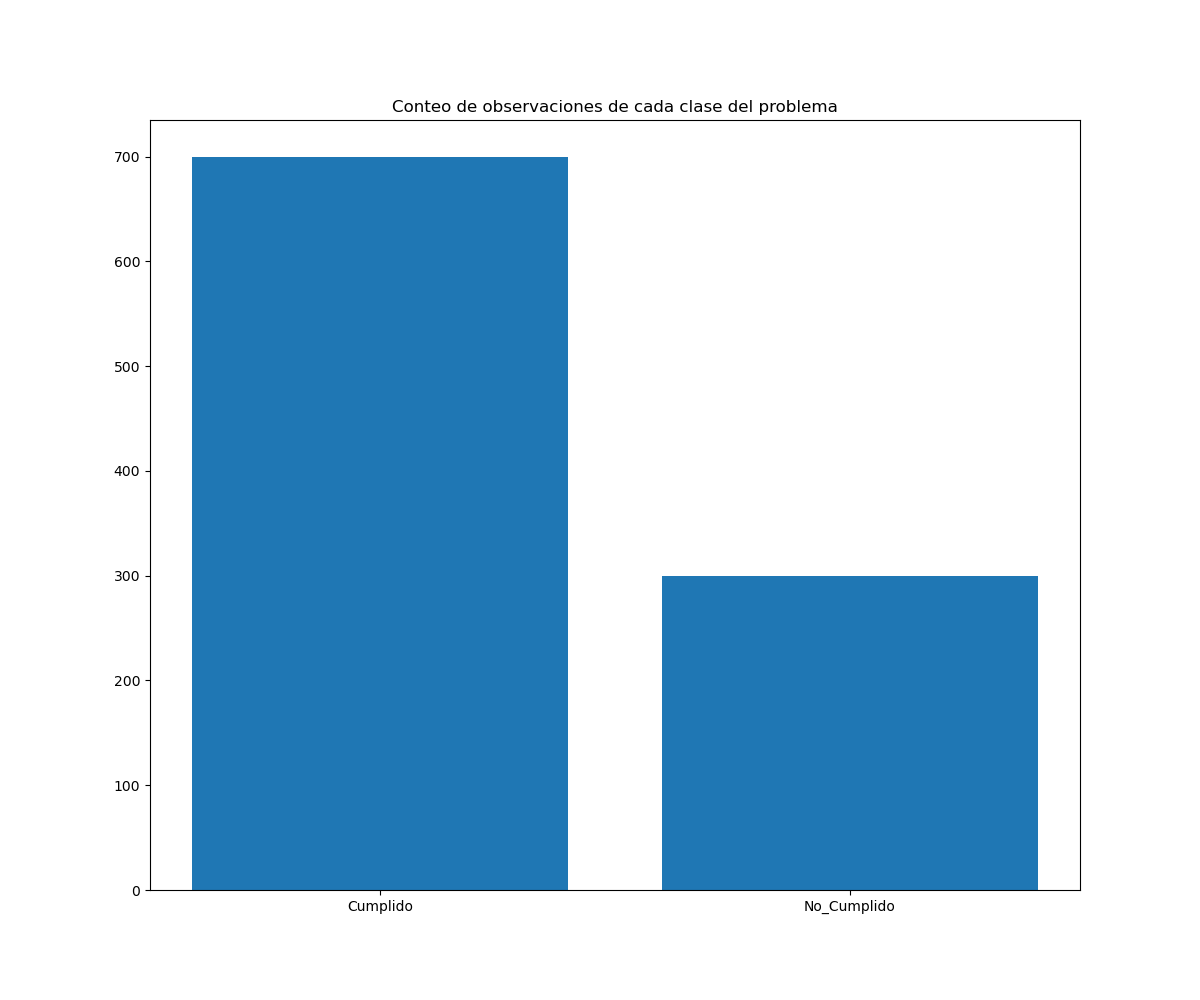
\includegraphics[scale = 0.6]{conteo_clases.png}
	\caption{Conteo de observaciones para cada clase del problema.}
	\label{fig:conteo_clases}
\end{figure}

Como podemos ver, en este caso no contamos con un número similar de observaciones en cada clase, teniendo en la clase donde no se han cumplido los pagos menos de la mitad de observaciones que en la clase donde si. Este problema lo podríamos solucionar intentando obtener más muestras o aplicando un sobremuestreo con técnicas como SMOTE o ADASYN, sin embargo no es el objetivo de la asignatura y por lo tanto se ha trabajado con el conjunto dado.

También se ha obtenido la matriz de correlaciones entre predictores, ya que es interesante saber si dos predictores están muy correlados de cara a saber si aportan la misma información y por lo tanto podríamos eliminar uno de ellos:

\begin{figure}[H]
	\centering
	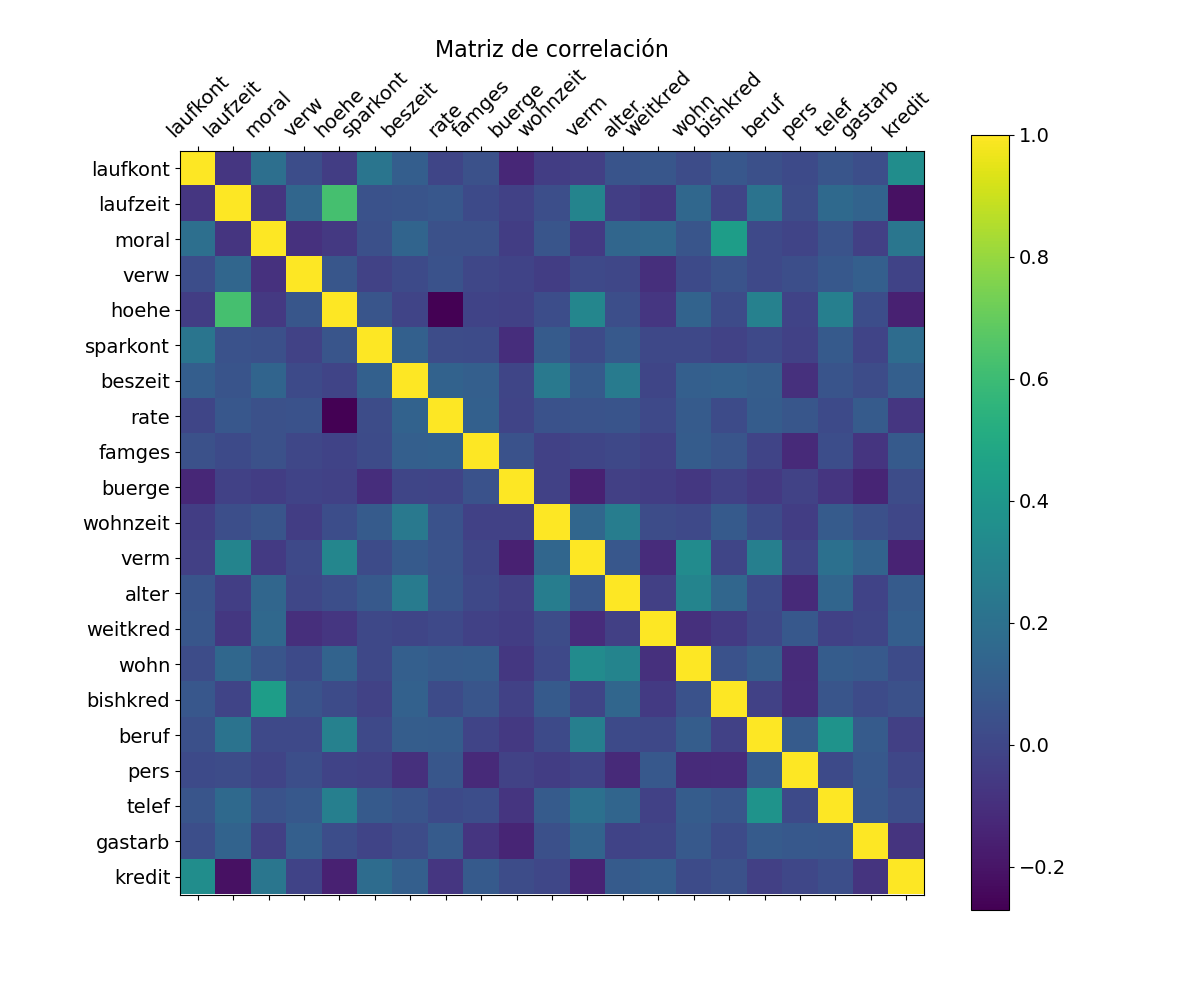
\includegraphics[scale = 0.6]{matriz_correlacion.png}
	\caption{Matriz de correlación entre las variables del problema.}
	\label{fig:matriz_correlacion}
\end{figure}

En este caso no existe una correlación muy alta entre ninguno de los predictores.

Otra de las gráficas de interés obtenidas es una gráfica con la distribución de cada predictor, ya que en este caso vamos a aplicar PCA, técnica que asume que las variables siguen una distribución normal y, aunque podemos aplicar esta técnica sin que esto se cumpla, obtendremos mejores resultados si esto es cierto:

\begin{figure}[H]
	\centering
	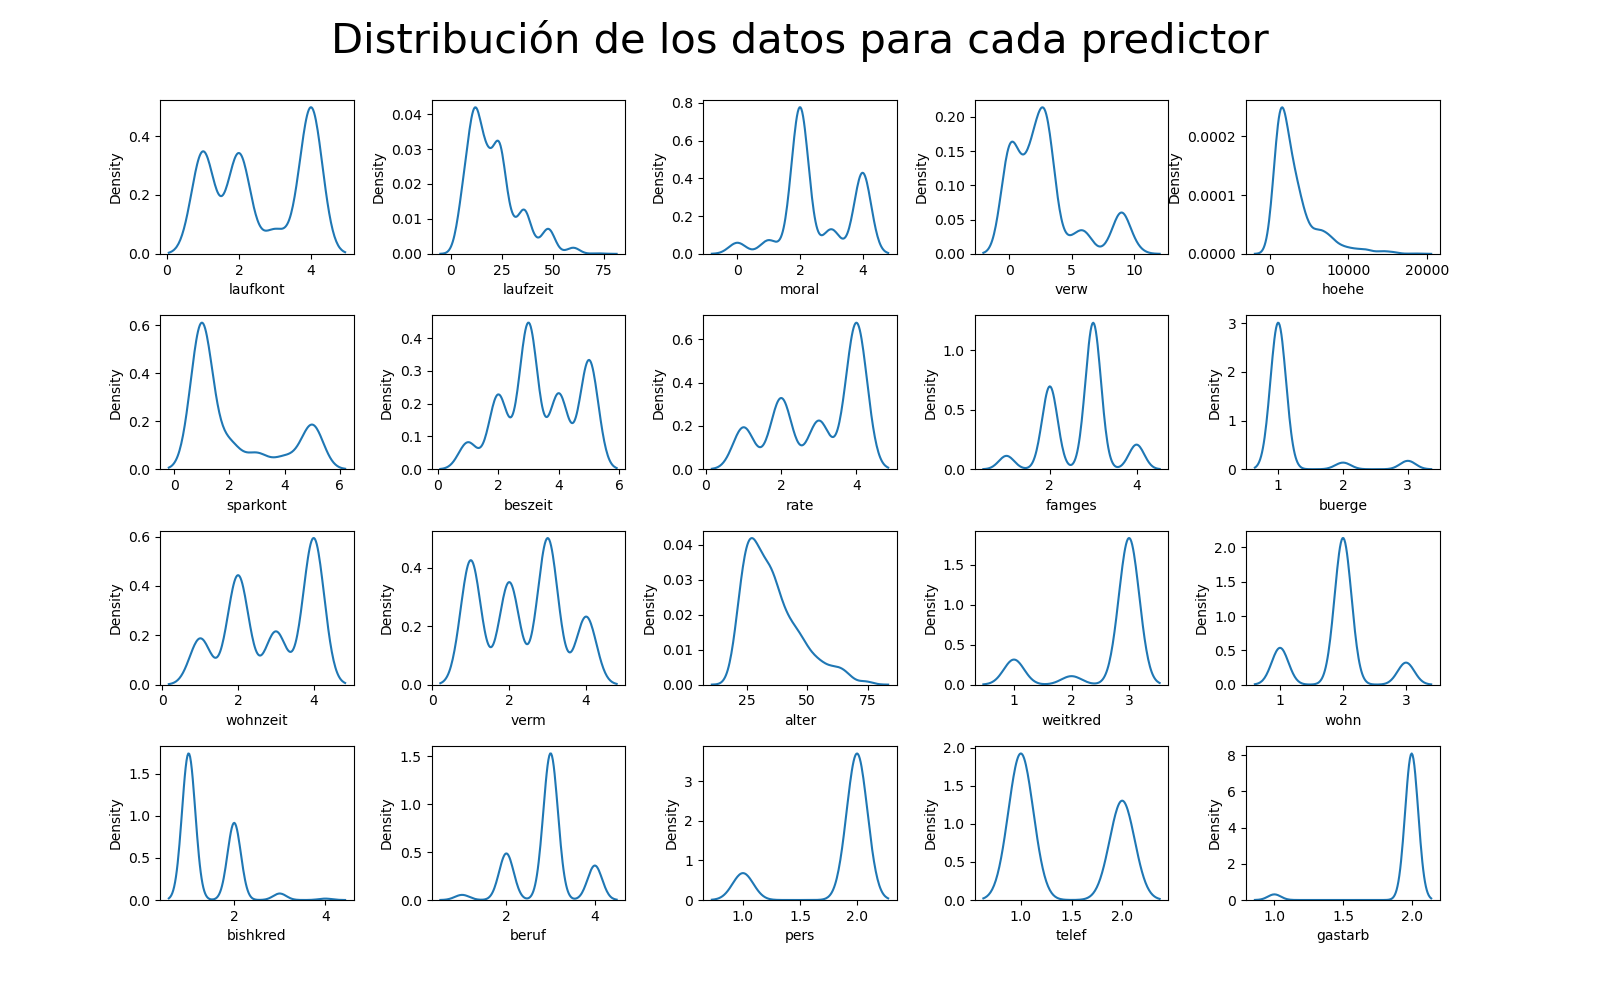
\includegraphics[scale = 0.4]{distribucion_variables.png}
	\caption{Distribución de las variables del problema.}
	\label{fig:distribucion_variables}
\end{figure}

Para nuestro problema vemos que ninguno de nuestros predictores sigue una distribución normal, aunque aun así vamos a intentar aplicar la reducción de dimensionalidad con PCA.



\newpage


\section{Preprocesamiento}

Antes de trabajar con los datos tenemos que aplicar cierto preprocesamiento para que se comporten de forma adecuada con el modelo que intentará predecir la clase.


La primera transformación que aplicaremos será una normalización. Debido a que los datos están en rangos de valores muy distintos y algunas de las técnicas que utilizaremos tendrán en cuenta valores como las distancias, es necesario escalar los datos para que no dar más importancia a un predictor simplemente porque sus valores son más grandes que los del resto.

Para aplicar esta transformación utilizaremos una normalización de media cero y desviación uno aplicando el método \texttt{StandardScaler} de scikit-learn.

Tras esta normalización pasaremos a aplicar el análisis de componentes principales con el método \texttt{PCA} disponible en scikit-learn. De cara a buscar un mejor espacio para la clasificación, se ha pasado como parámetro a este modelo que mantenga los suficientes datos como para explicar el 90\% de la varianza, obteniendo como resultado dieciséis nuevos predictores.

De cara a visualizar el resultado se ha creado una gráfica donde se visualiza la clase de las observaciones dependiendo de los dos nuevos predictores que más varianza explican, un poco más del 20\%:

\begin{figure}[H]
	\centering
	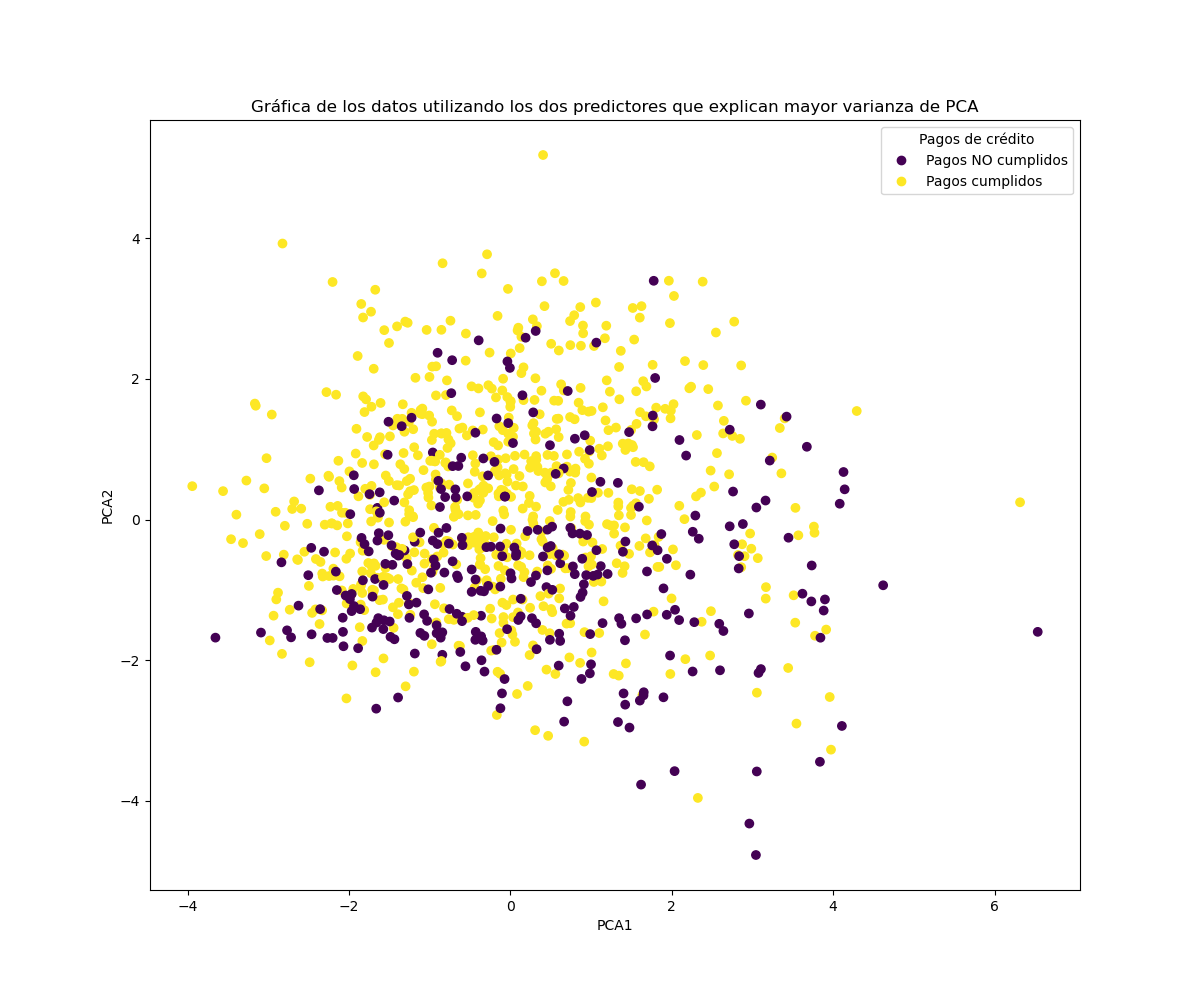
\includegraphics[scale = 0.6]{datos_pca.png}
	\caption{Observaciones en función de los dos mejores predictores tras PCA.}
	\label{fig:datos_pca}
\end{figure}

Como vemos sigue existiendo demasiado solape como para ver una distinción clara entre las clases, sin embargo esto es solo utilizando dos de los dieciséis predictores obtenidos por PCA.

\newpage


\section{Modelos a utilizar}

De cara a resolver este problema utilizaremos los siguientes modelos:

\begin{itemize}
	\item Regresión Logsitica.
	\item Árbol de decisión.
	\item Random Forest.
	\item Máquinas de soporte de vectores (SVM).
	\item Multi Layer Perceptron.
\end{itemize}


De cara a buscar los mejores hiperparámetros para estos modelos realizaremos una búsqueda de hiperparámetros como veremos en el siguiente apartado.

\section{Búsqueda de hiperparámetros}

Para realizar esta búsqueda de hiperparámetros se han saleccionado distintos valores para cada parámetro de todos los modelos a utilizar, y utilizando tanto GridSearchCV como RandomizedSearchCV se han obtenido los mejores hiperparámetros para cada modelo.

El espacio de búsqueda de todos los parámetros se puede ver en el código adjunto a esta memoria.

Debido a que esta búsqueda de hiperparámetros es muy lenta, en especial en el caso de GridSearchCV ya que este método recorre todas las posibles combinaciones, es posible ejecutar el script con el parámetro \texttt{cargar\_modelos} para que utilizando pickle cargue los modelos escogidos en una ejecución anterior. Si no es capaz de cargar estos modelos, o no se le pasa este parámetro, realizará la búsqueda de hiperparámetros y almacenará los resultados en la carpeta \texttt{modelos}.

\begin{lstlisting}
python proyecto.py cargar_modelos
\end{lstlisting}

\subsection{Mejores hiperparámetros obtenidos por GridSearchCV}


\subsection{Mejores hiperparámetros obtenidos por RandomizedSearchCV}


\section{Métodos de validación}

De cara a validar los resultados se ha realizado tanto una separación en entrenamiento y test, además de utilizar validación cruzada en el entrenamiento. De esta forma, con los resultados de validación cruzada podemos comprobar si el modelo bien o sobreaprende los datos, mientras que con el conjunto de test podemos comprobar como funciona para datos con los que no ha entrenado.

Para realizar esto se ha realizado una función que recibe el modelo a entrenar, los datos, el número de folds para validación cruzada, y el porcentaje de datos que queremos dejar en test.

Si no se indica conjunto de test, se obtiene utilizando el porcentaje dado a partir del parámetro, y tras esta separación se aplica la función \texttt{cross\_validate} de scikit-learn para entrenar el modelo con validación cruzada.

Tras esto se obtiene la media de precisión del modelo en validación cruzada, así como la precisión en el conjunto de test utilizando el mejor modelo obtenido de la validación cruzada.

\section{Resultados}


\end{document}
